\section{Overordnet arkitektur}
\label{sec:arkitektur}

VideoAPI er organisert som en lagdelt arkitektur, vist i figur~\ref{fig:lagarkitektur}. Lagdelingen skiller HTTP-håndtering, forretningslogikk og backend-integrasjon fra hverandre, noe som reduserer koblingen mellom delene av systemet og gjør det enklere å endre én del uten å påvirke resten.

\usetikzlibrary{positioning,arrows.meta}
\begin{figure}[htbp]
\centering
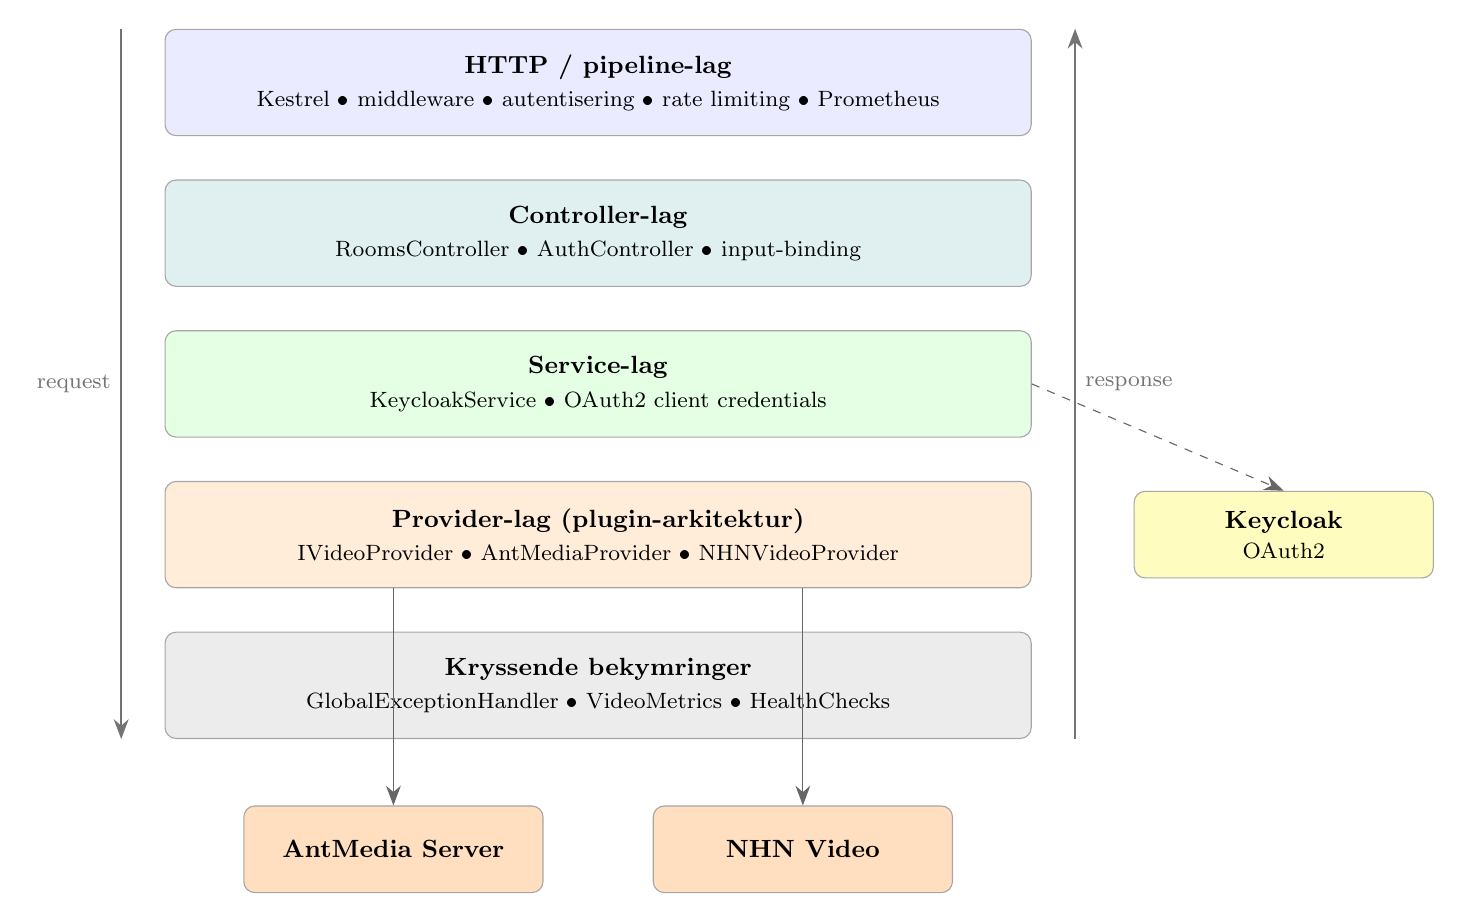
\begin{tikzpicture}[
    >={Stealth[length=2.5mm]},
    node distance=0.55cm,
    layer/.style={
        draw=black!35,
        line width=0.4pt,
        rounded corners=4pt,
        minimum width=11cm,
        minimum height=1.35cm,
        text centered,
        align=center,
        inner sep=6pt,
        font=\small
    },
    ext/.style={
        draw=black!35,
        line width=0.4pt,
        rounded corners=4pt,
        minimum width=3.8cm,
        minimum height=1.1cm,
        text centered,
        align=center,
        inner sep=4pt,
        font=\small
    },
    arrowlbl/.style={font=\footnotesize\color{black!65}}
]

% --- Layers (top to bottom) ---
\node[layer, fill=blue!8]                  (http)  {\textbf{HTTP / pipeline-lag}\\[1pt]
    {\footnotesize Kestrel \textbullet{} middleware \textbullet{} autentisering \textbullet{} rate limiting \textbullet{} Prometheus}};
\node[layer, fill=teal!12, below=of http]  (ctrl)  {\textbf{Controller-lag}\\[1pt]
    {\footnotesize RoomsController \textbullet{} AuthController \textbullet{} input-binding}};
\node[layer, fill=green!10, below=of ctrl] (svc)   {\textbf{Service-lag}\\[1pt]
    {\footnotesize KeycloakService \textbullet{} OAuth2 client credentials}};
\node[layer, fill=orange!15, below=of svc] (prov)  {\textbf{Provider-lag (plugin-arkitektur)}\\[1pt]
    {\footnotesize IVideoProvider \textbullet{} AntMediaProvider \textbullet{} NHNVideoProvider}};
\node[layer, fill=gray!15, below=of prov]  (cross) {\textbf{Kryssende bekymringer}\\[1pt]
    {\footnotesize GlobalExceptionHandler \textbullet{} VideoMetrics \textbullet{} HealthChecks}};

% --- External backends at the bottom ---
\node[ext, fill=orange!25] (ant) at ([xshift=-2.6cm, yshift=-1.4cm]cross.south) {\textbf{AntMedia Server}};
\node[ext, fill=orange!25] (nhn) at ([xshift= 2.6cm, yshift=-1.4cm]cross.south) {\textbf{NHN Video}};

% --- External service on the right (Keycloak), aligned with Service-lag ---
\node[ext, fill=yellow!25] (kc) at ([xshift=3.2cm]prov.east) {\textbf{Keycloak}\\{\footnotesize OAuth2}};


% --- Request arrow (left, downward) ---
\draw[->, thick, black!55]
    ([xshift=-0.55cm]http.north west) -- ([xshift=-0.55cm]cross.south west)
    node[midway, left, arrowlbl] {request};

% --- Response arrow (right of layer stack, upward) ---
\draw[->, thick, black!55]
    ([xshift=0.55cm]cross.south east) -- ([xshift=0.55cm]http.north east)
    node[midway, right, arrowlbl] {response};
    
% --- Provider to backends ---
\draw[->, black!60] (prov.south -| ant.north) -- (ant.north);
\draw[->, black!60] (prov.south -| nhn.north) -- (nhn.north);

% --- Service to Keycloak (dashed) ---
\draw[->, dashed, black!60] (svc.east) -- (kc.north);

\end{tikzpicture}
\caption{Overordnet lagarkitektur for HDO VideoAPI.}
\label{fig:lagarkitektur}
\end{figure}


\begin{description}
    \item[HTTP-pipeline-laget] håndterer innkommende trafikk og inneholder middleware for blant annet unntakshåndtering, HTTPS, \gls{cors}, rate limiting, JWT-autentisering, autorisasjon og Prometheus-metrikker. Disse mekanismene er lagt i pipelinen fordi de gjelder hele API-et, ikke én spesifikk romoperasjon.
    
    \item[Controller-laget] fungerer som et tynt bindeledd mellom HTTP-kontrakten og provider-laget. Controllerne binder innkommende forespørsler, velger riktig provider og returnerer HTTP-svar, men inneholder ikke backend-spesifikk logikk. Slik kan API-kontrakten holdes stabil selv om integrasjonen mot AntMedia eller NHN endres.
    
    \item[Provider-laget] er kjernen i arkitekturen. Resten av applikasjonen forholder seg til et felles \texttt{IVideoProvider}-grensesnitt, mens AntMedia- og NHN-spesifikk logikk holdes i egne provider-implementasjoner.
    
    \item[Service-laget] inneholder hjelpetjenester som brukes på tvers av provider-implementasjonene, særlig \texttt{KeycloakService} som håndterer uthenting og caching av tilgangstoken fra Keycloak.
    
    \item[Kryssende bekymringer] som feilhåndtering, metrikker og helsesjekker behandles utenfor kjerneflyten for romoperasjoner. Arkitekturen er også stateless: API-et lagrer ikke videorom eller sesjonsdata mellom forespørsler, men lar slik tilstand ligge hos de eksterne videomotorene. Dette støtter horisontal skalering og er i tråd med krav~I1.2~\cite{hdo_kravspec}.
\end{description}
\newpage
\begin{lstlisting}[language=CSharp, caption={Oppstartskonfigurasjon delegert til navngitte extension-metoder}, label={lst:program-startup}]
// HDO-VideoAPI/Program.cs

var builder = WebApplication.CreateBuilder(args);

// Konfigurasjon
builder.Configuration.AddEnvironmentVariables();            // Miljøvariabler
builder.ConfigureVideoHosting();                            // Kestrel og HTTPS

// Tjenester registreres per ansvarsdomene
builder.Services.AddVideoRateLimiting();                    // Hastighetsbegrensning
builder.Services.AddVideoApiCore();                         // Controllers, JSON, OpenAPI
builder.Services.AddVideoCors(builder.Configuration);       // CORS-policy
builder.Services.AddVideoProviders(builder.Configuration);  // Plugin-arkitektur
builder.Services.AddVideoHealthChecks(builder.Environment); // Helsesjekker 
builder.Services.AddVideoKeycloak(builder.Configuration);   // OAuth2/JWT

// Bygg og start applikasjonen
var app = builder.Build();
app.UseVideoApi();
app.Run();
\end{lstlisting}
Kodeliste~\ref{lst:program-startup} viser hvordan oppstarten er holdt kompakt ved å delegere konfigurasjon til navngitte extension-metoder. Dette gjør \texttt{Program.cs} til en oversikt over systemets hovedmoduler, i stedet for å samle all konfigurasjon i én fil.